\section{Results}
\label{sec:results}

As a result of our work, we believe to have found new motivation to continue pushing area in the research of Raft variants aimed at use in large-scale systems in practice.
When we originally planned for this project, we were focused primarly about exploring the results of such work. 
Due to our cirucmstances however we were unable to gather the diverse and fine-grained data that we originally planned.
The scope of the project was a lot larger than we intended, which caused most of our research to be based on the specification changes.
However as a result of the broad scope of this project, we hope to motivate further work that is able to properly test
 and improve upon these ideas. We firmly believe that there is still much progress to be explored in the world of practical consensus. 

\begin{figure}[h!]
    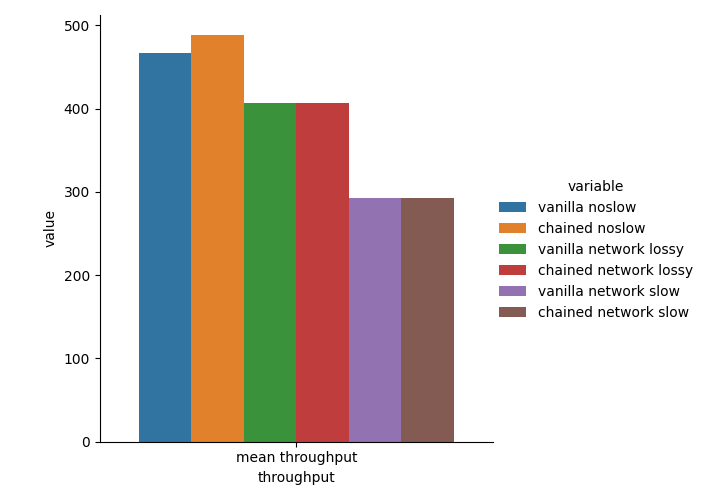
\includegraphics[width=\linewidth]{comparison_mean_throughput.png}
    \caption{Mean Throughput}
    \label{fig:comp_thput}
\end{figure}
\begin{figure}[h!]
    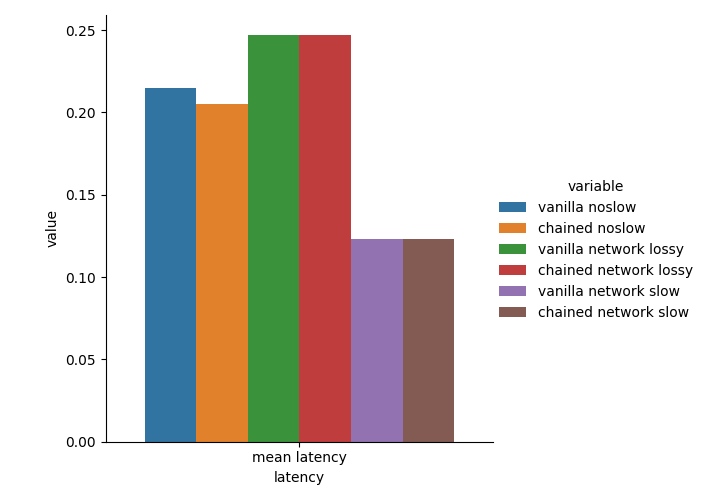
\includegraphics[width=\linewidth]{comparison_mean_latency.png}
    \caption{Mean Latency}
    \label{fig:comp_lat}
\end{figure}

During our benchmarks, we were able to find slight throughput and latency gains for Flexible Chained Raft over Raft. 
We assume most of this is because of the flexible quorums, but we were also surprised to find our chained implementation not causing performance overhead. 
Chained blocks allow the leader to easily send all log entries to each node every RPC call. As soon as a follower finds the tail of the block in the message in its local block chain - it is able to append the whole chain.
This decreases the messages the leader has to send, with the tradeoff of on average longer messages (and thus higher communication complexity overall). 
We also found that during implementation, it was quite easy to resolve bugs in the implementation due to the immutable structure of the block-chain.
Overall, we are quite excited in the results, specifically for the chained implementation, and believe that much further research can be done in this area.
We hope to eventually extend and perhaps finalize this work in a later project where we can explore the behavior and benefits of the immutable log structure in finer details. 

\begin{figure}[h!]
    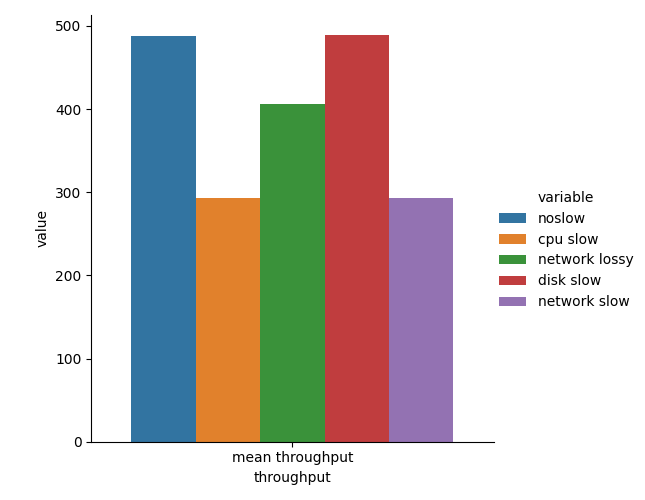
\includegraphics[width=\linewidth]{chained_mean_throughput.png}
    \caption{Mean Throughput for Chained Raft}
    \label{fig:chain_thput}
\end{figure}
\begin{figure}[h!]
    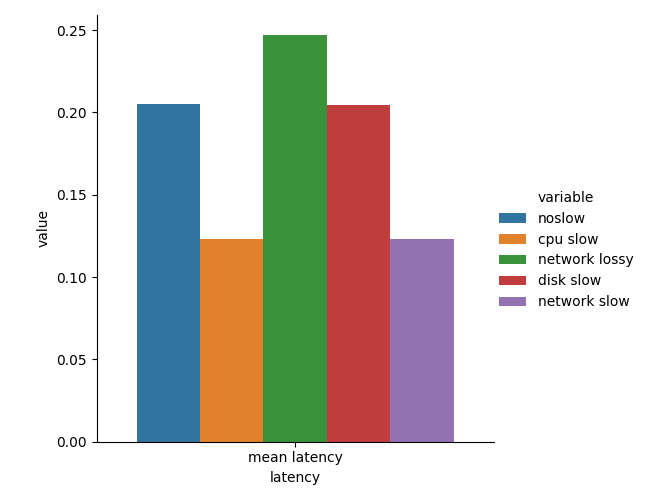
\includegraphics[width=\linewidth]{chained_mean_latency.png}
    \caption{Mean Latency for Chained Raft}
    \label{fig:chain_lat}
\end{figure}

During fault-injection benchmarks we saw that both implementations performed quite similarly under the more fine-grained faults that we tested.
Specifically, under certain fail-slow faults (namely cpu slow and network slow) we saw massive throughput drops which equalized the implementations. 
This is because the clients that were communicating to the faulty nodes were no longer able to get valid responses in time, and thus achieved no throughput.
Disk slow faults did not bottleneck the workload despite the heavy write workload, as for both implementations it's performance trended closely with no slow injections.
This was interesting, but also gives us the idea that of all things to bottleneck in a distributed consensus node, it may be hardest to bottleneck disk write speed. 
There are much more frequent operations that are being executed, which are much more costly in terms of time. 
We imagine that with larger services with write heavy workloads built on top of the consensus cluster, such a fault would be much more damaging to performance.

Overall, we have seen that with flexible chained raft one can potentially see a performance gain under normal network behavior.
We reasoned the potential benefits of using immutable block-chain based RPC's in Raft, both for easier implementation and observation.




